%% LyX 2.2.3 created this file.  For more info, see http://www.lyx.org/.
%% Do not edit unless you really know what you are doing.
\documentclass[spanish]{article}
\usepackage[T1]{fontenc}
\usepackage[utf8]{luainputenc}
\usepackage{geometry}
\geometry{verbose,tmargin=2cm,bmargin=2cm,lmargin=2cm,rmargin=2cm,headheight=2cm,headsep=2cm}
\setlength{\parindent}{0bp}
\usepackage{float}
\usepackage{textcomp}
\usepackage{amstext}
\usepackage{graphicx}

\makeatletter

%%%%%%%%%%%%%%%%%%%%%%%%%%%%%% LyX specific LaTeX commands.
%% Because html converters don't know tabularnewline
\providecommand{\tabularnewline}{\\}

\makeatother

\usepackage{babel}
\addto\shorthandsspanish{\spanishdeactivate{~<>}}

\begin{document}

\section{Comportamiento de Amplificador Operacional Inversor}

A lo largo de esta seccion se procedera a analizar el comportamiento
ideal y real del amplificador operacional \emph{LM324 }conectado como
se muestra en la figura \ref{1_a_1}. Considerando los valores de
los componentes como se puede ver en la tabla \ref{1_a_t_1}. Es necesario
aclarar que para realizar cualquier calculo numérico y simbolico de
ecuaciones se utilizo la librería \emph{SymPy }de python, por lo tanto
si no se encuentra el procedimiento para el hallazgo de una ecuación
en este informe, es porque se halló mediante programación con variables
simbólicas.

\begin{figure}[H]
\begin{centering}
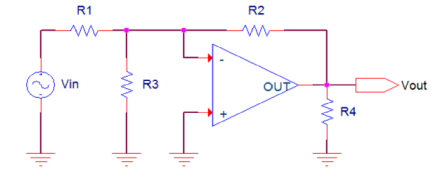
\includegraphics[scale=0.75]{Resources1a/Circuito1a}
\par\end{centering}
\caption{Circuito a analizar}
\label{1_a_1}
\end{figure}

\begin{table}[H]
\begin{centering}
\begin{tabular}{|c|c|c|c|}
\hline 
Caso & $R_{1}=R_{3}$ & $R_{2}$ & $R_{4}$\tabularnewline
\hline 
\hline 
1 & $10\left(k\Omega\right)$ & $100\left(k\Omega\right)$ & $40\left(k\Omega\right)$\tabularnewline
\hline 
2 & $10\left(k\Omega\right)$ & $10\left(k\Omega\right)$ & $40\left(k\Omega\right)$\tabularnewline
\hline 
3 & $100\left(k\Omega\right)$ & $10\left(k\Omega\right)$ & $400\left(k\Omega\right)$\tabularnewline
\hline 
\end{tabular}
\par\end{centering}
\caption{Valores de los componentes}
\label{1_a_t_1}

\end{table}

\subsection{Transferencia\label{subsec:1_a_1}}

Comenzando por el analisis ideal, se pidió calcular y graficar la
relación $\frac{V_{out}}{V_{in}}$, esto quiere decir, considerando
$a_{0}$ finito y $A(\omega)$ con polo dominante. Considerando las
siguientes ecuaciones descriptas a continuacion y operando correctamente,
se llega a que la relacion $\frac{V_{out}}{V_{in}}$ esta dada por
la ecuación (\ref{eq:1_a_1}).

\[
\left\{ \begin{array}{c}
V_{out}=-A(\omega)v^{-}\\
I=i_{3}+i_{1}\\
i_{1}=-i_{2}\\
v^{-}=i_{3}R_{3}\\
V_{in}-IR_{1}=v^{-}
\end{array}\right.
\]

\begin{equation}
H(s)=\frac{V_{out}}{V_{in}}=-\frac{R_{2}R_{3}Wa_{0}}{R_{1}R_{2}\left(W+s\right)+R_{1}R_{3}Wa_{0}+R_{1}R_{3}\left(W+s\right)+R_{2}R_{3}\left(W+s\right)}\label{eq:1_a_1}
\end{equation}

\[
H(s)=-\frac{5\cdot10^{15}}{2.1\,10^{9}s+502\,10^{12}}\,Caso\,1
\]

\[
H(s)=-\frac{502\,10^{12}}{300\,10^{6}s+502\,10^{12}}\,Caso\,2
\]

\[
H(s)=-\frac{5\cdot10^{15}}{12\,10^{9}s+5\cdot10^{16}}\,Caso\,3
\]

Como podemos ver, tenemos un polo en nuestra transferencia por lo
cual, el circuito se deberia comportar a grandes rasgos como un pasabajos.
Es importante notar, que el valor de $R_{4}$ no afecta a la transferencia
del circuito. Si graficamos la transferencia de el circuito para los
distintos casos, podemos ver que, en efecto, se comporta como un pasabajos,
con diferente frecuencia de corte $f_{0}$, esto se puede ver en las
figurar \ref{1_a_2}, \ref{1_a_2_b} y \ref{1_a_2_c}. La diferencia
con lo simulado se debe a que la frecuencia del polo dominante dada
por la hoja de datos no esta bien especificada, y en la calculada
se uso un polo dominante de 7,5 (Hz) (Que era lo que se observaba
aproximadamente en el grafico provisto por el graficante) y en el
simulado se uso el modelo real del LM324.

\begin{figure}[H]
\begin{centering}
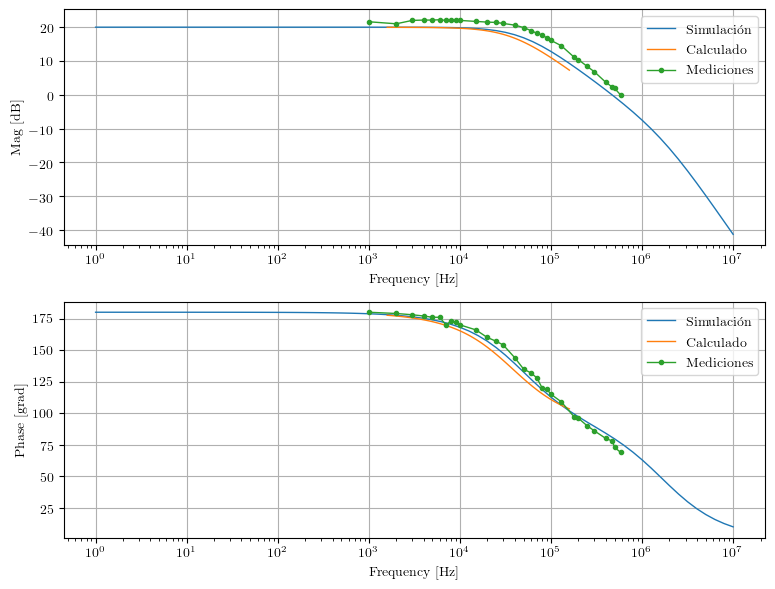
\includegraphics[scale=0.5]{Resources1a/H1}
\par\end{centering}
\caption{Comportamiento del circuito para el caso 1}
\label{1_a_2}
\end{figure}

\begin{figure}[H]
\begin{centering}
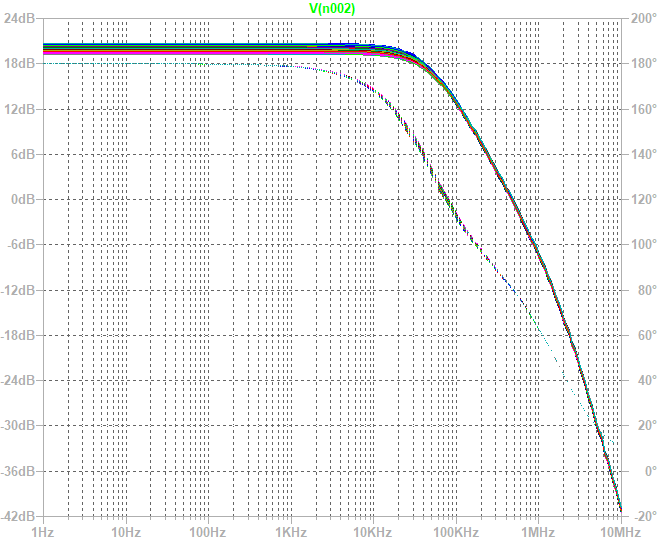
\includegraphics[scale=0.5]{Resources1a/montecarlo1a_1}
\par\end{centering}
\caption{Análisis montecarlo del circuito para el caso 1}

\end{figure}

\begin{figure}[H]
\begin{centering}
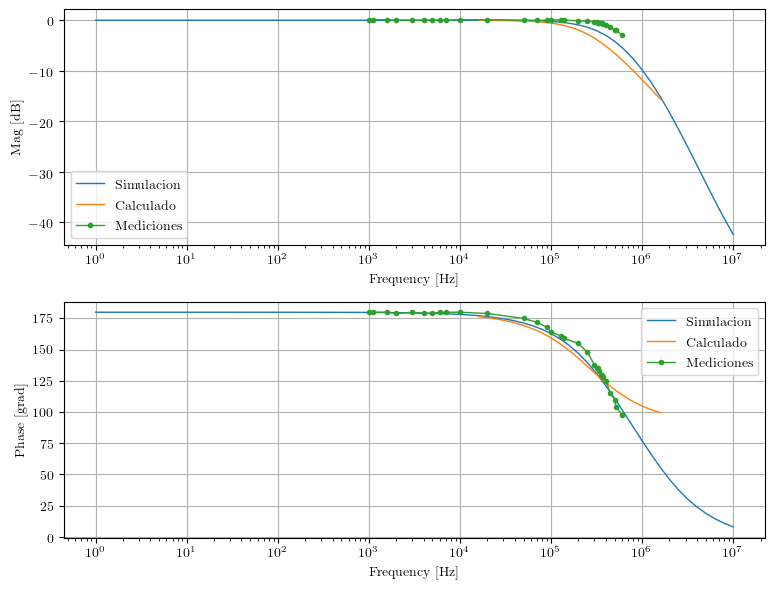
\includegraphics[scale=0.5]{Resources1a/H2}
\par\end{centering}
\caption{Comportamiento del circuito para el caso 2}
\label{1_a_2_b}
\end{figure}

\begin{figure}[H]
\begin{centering}
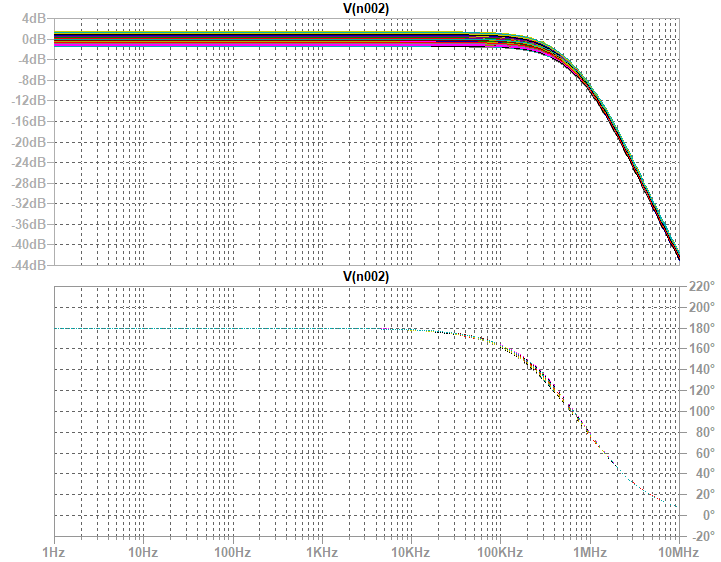
\includegraphics[scale=0.5]{Resources1a/montecarlo1a_2}
\par\end{centering}
\caption{Análisis montecarlo del circuito para el caso 2}

\end{figure}

\begin{figure}[H]
\begin{centering}
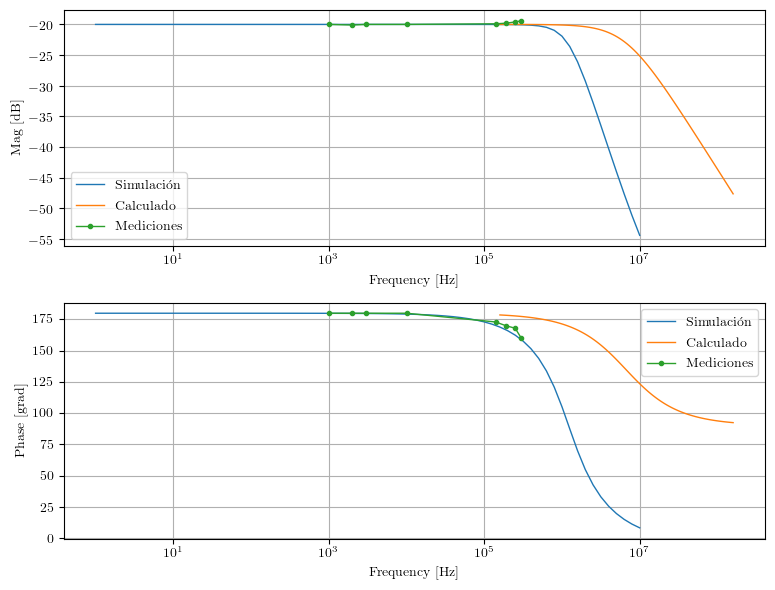
\includegraphics[scale=0.5]{Resources1a/H3}
\par\end{centering}
\caption{Comportamiento del circuito para el caso 3}
\label{1_a_2_c}

\end{figure}

\begin{figure}[H]
\begin{centering}
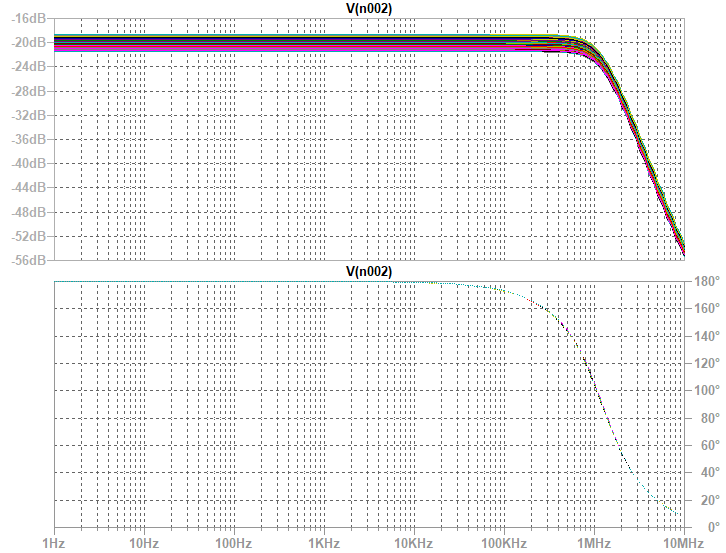
\includegraphics[scale=0.5]{Resources1a/montecarlo1a_3}
\par\end{centering}
\caption{Análisis montecarlo del circuito para el caso 3}

\end{figure}

Como se pudo observar en las Figuras \ref{1_a_2}, \ref{1_a_2_b}
y \ref{1_a_2_c}, para el caso 1, el circuito se comporta como un
amplificador de 20(dB), hasta la frecuencia del polo, donde ya empieza
a afectar el comportamiento de pasabajos. Un comportamiento similar
tuvieron los casos 2 y 3, con la salvedad de que en el caso 2 se trataba
de un buffer y en el caso 3 de un atenuador de 20(dB).

\subsection{Impedancia de entrada\label{subsec:1_a_2}}

Consecuentemente, se nos instó a calcular la impedancia de entrada
vista por el generador hacia nuestro circuito. Nuevamente, utilizando
las ecuaciones descriptas en la previa subseccion, y operando adecuadamente,
llegamos a que la impedancia de entrada es la descripta en la ecuación
(\ref{eq:1_a_2}).

\[
K=\frac{R_{2}a_{0}\omega_{p}(R_{3}+R_{1})-\omega_{p}(a_{0}-1)\left(R_{2}R_{3}+R_{1}R_{2}+R_{1}R_{3}\right)}{R_{2}a_{0}\omega_{p}-\left(R_{2}+R_{3}\right)\omega_{p}\left(a_{0}-1\right)}
\]

\[
C=\frac{\omega_{p}(a_{0}-1)\left(R_{2}R_{3}+R_{1}R_{2}+R_{1}R_{3}\right)-R_{2}a_{0}\omega_{p}\left(R_{3}+R_{1}\right)}{\left(R_{2}R_{3}+R_{1}R_{2}+R_{1}R_{3}\right)}
\]

\[
L=\frac{\left(R_{2}+R_{3}\right)\omega_{p}\left(a_{0}-1\right)-R_{2}a_{0}\omega_{p}}{R_{2}+R_{3}}
\]

\begin{equation}
\Rightarrow Z_{in}=K\,\frac{1+\frac{s}{C}}{1+\frac{s}{L}}\label{eq:1_a_2}
\end{equation}

Por lo tanto, para cada caso tendremos una impedancia de entrada como
se muestra en las siguientes formulas:

\[
Z_{in}=\frac{912\times10^{3}f^{2}+100\times10^{12}}{47.77f^{2}+10\text{\texttimes}10^{9}}+i\frac{6.28\text{\texttimes}10^{9}f}{47.77f^{2}+10\text{\texttimes}10^{9}}\,\,\,Caso\,1
\]

\[
Z_{in}=\frac{5.92\times10^{3}f^{2}+25\text{\texttimes}10^{12}}{0.39f^{2}+2.5\text{\texttimes}10^{9}}+i\frac{157\text{\texttimes}10^{6}f}{0.39f^{2}+2.5\text{\texttimes}10^{9}}\,\,\,Caso\,2
\]

\[
Z_{in}=\frac{5.21\text{\texttimes}10^{6}f^{2}+100\text{\texttimes}10^{15}}{47.77f+999.98\text{\texttimes}10^{9}}+i\frac{62.83\text{\texttimes}10^{9}f}{47.77f+999.98\text{\texttimes}10^{9}}\,\,\,Caso\,3
\]

Graficando la impedancia de entrada con respecto a la frecuencia de
entrada, se puede ver en la figura \ref{1_a_3}, como va variando
dependiendo de la frecuencia, es decir, no permanece constante. Nuevamente,
podemos observar como esta impedancia no es afectada por $R_{4}$.

\begin{figure}[H]
\begin{centering}
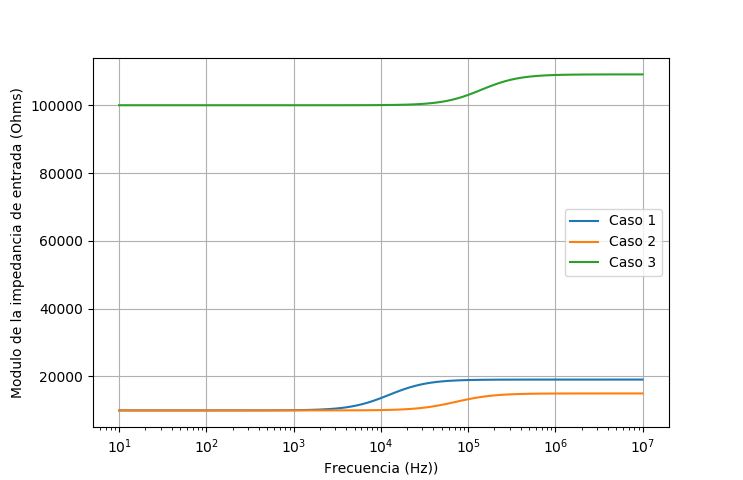
\includegraphics[scale=0.5]{Resources1a/zinpm}
\par\end{centering}
\begin{centering}
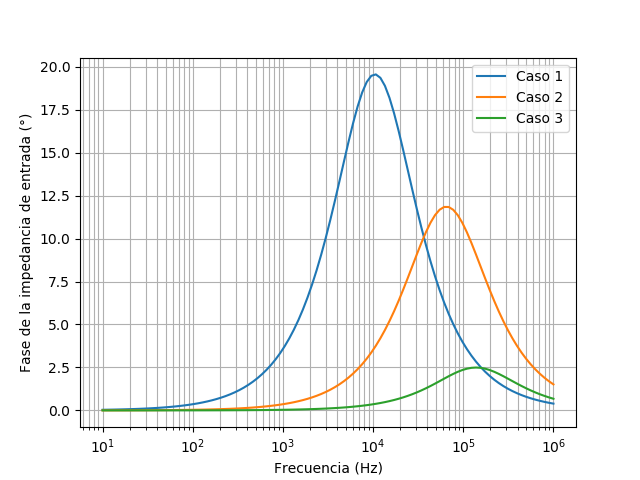
\includegraphics[scale=0.5]{Resources1a/zinpp}
\par\end{centering}
\caption{Impedancia de entrada Calculada}
\label{1_a_3}

\end{figure}

\begin{figure}[H]
\begin{centering}
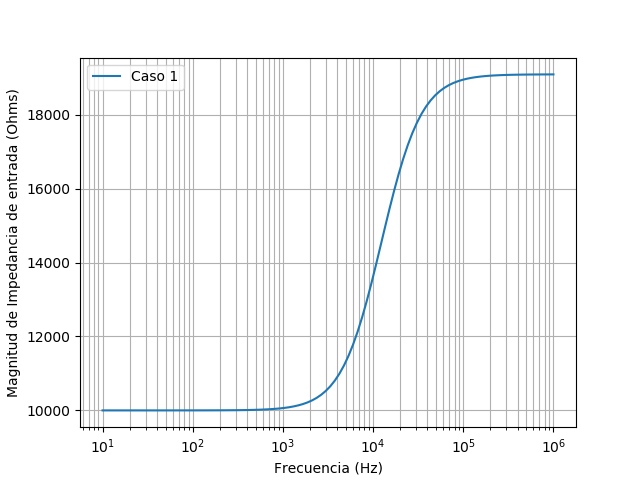
\includegraphics[scale=0.5]{Resources1a/zinpm1}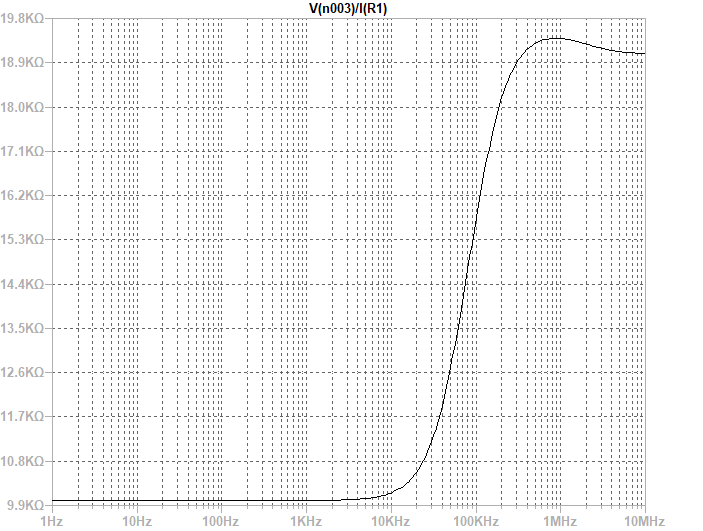
\includegraphics[scale=0.4]{Resources1a/zinpm1_sim}
\par\end{centering}
\caption{Calculo y simulación del modulo de la impedancia de entrada para el
caso 1}
\end{figure}

\begin{figure}[H]
\begin{centering}
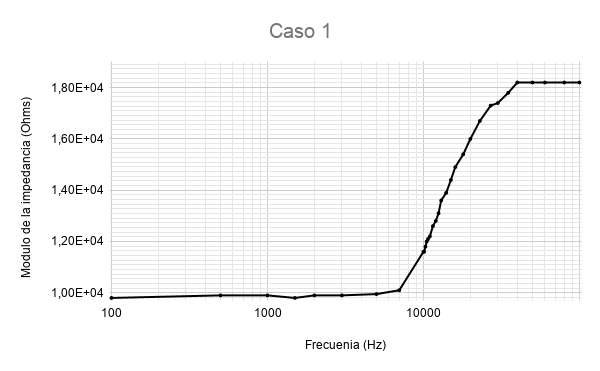
\includegraphics[scale=0.5]{Resources1a/zinpm1_med}
\par\end{centering}
\caption{Medición del modulo de la impedancia de entrada para el caso 1}

\end{figure}

\begin{figure}[H]
\begin{centering}
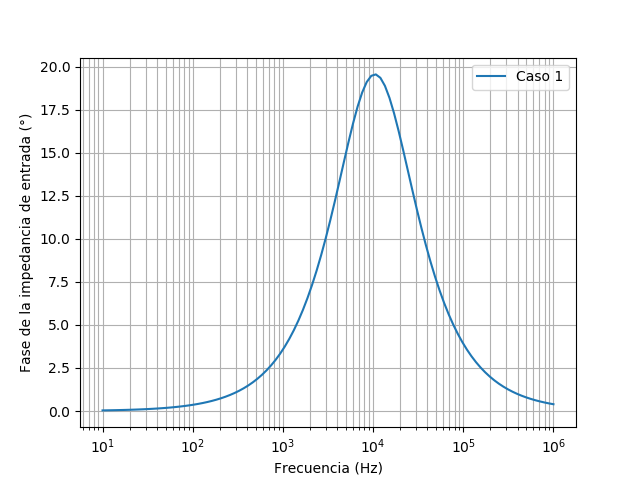
\includegraphics[scale=0.5]{Resources1a/zinpp1}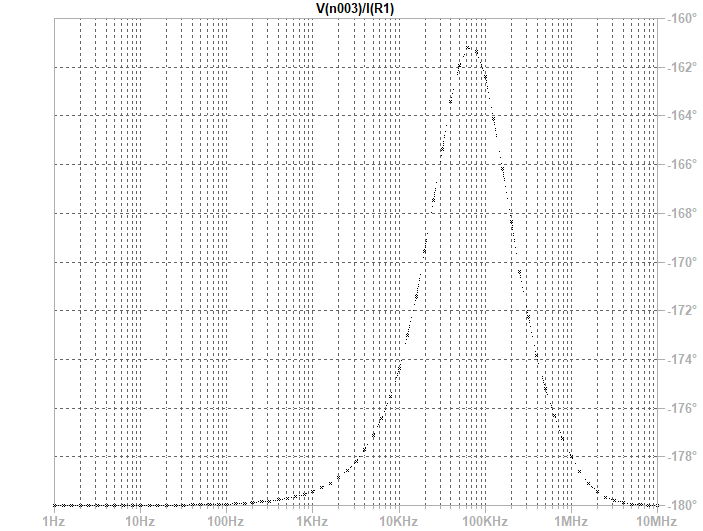
\includegraphics[scale=0.4]{Resources1a/zinpp1_sim}
\par\end{centering}
\caption{Calculo y simulación de la fase de la impedancia de entrada para el
caso 1}

\end{figure}

\begin{figure}[H]
\begin{centering}
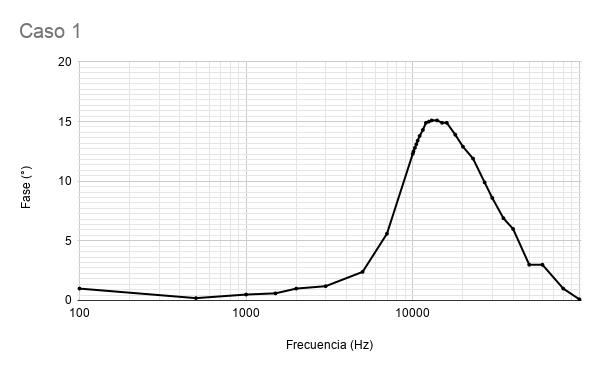
\includegraphics[scale=0.5]{Resources1a/zinpp1_med}
\par\end{centering}
\caption{Medición de la fase de la impedancia de entrada para el caso 1}

\end{figure}

\begin{figure}[H]
\begin{centering}
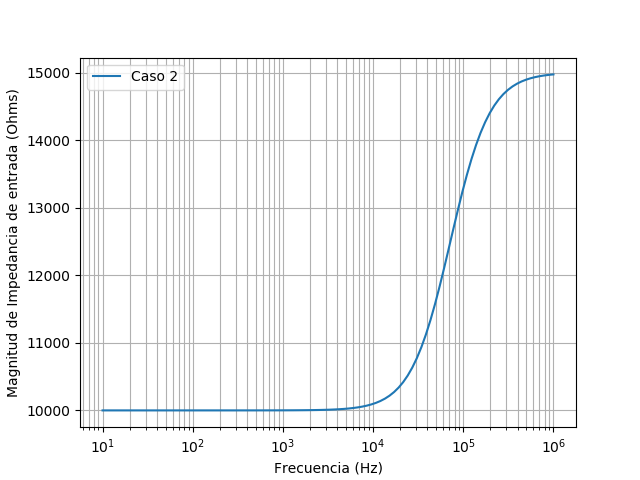
\includegraphics[scale=0.5]{Resources1a/zinpm2}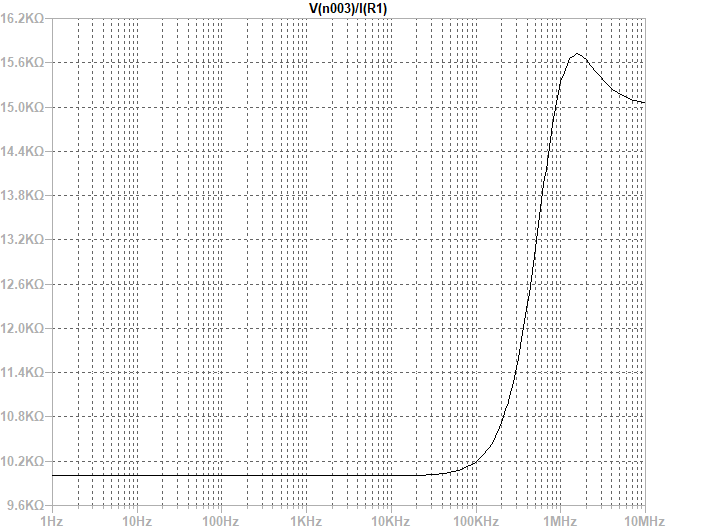
\includegraphics[scale=0.4]{Resources1a/zinpm2_sim}
\par\end{centering}
\caption{Calculo y simulación del modulo de la impedancia de entrada para el
caso 2}
\end{figure}

\begin{figure}[H]
\begin{centering}
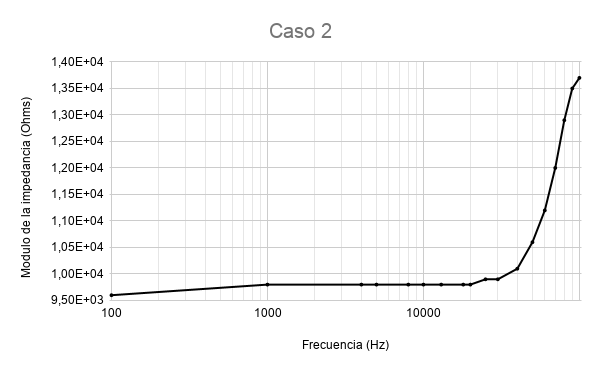
\includegraphics[scale=0.5]{Resources1a/zinpm2_med}
\par\end{centering}
\caption{Medición del modulo de la impedancia de entrada para el caso 2}

\end{figure}

\begin{figure}[H]
\begin{centering}
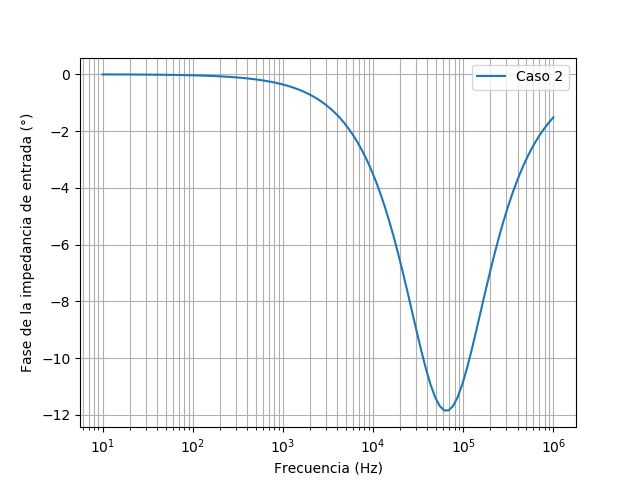
\includegraphics[scale=0.5]{Resources1a/zinpp2}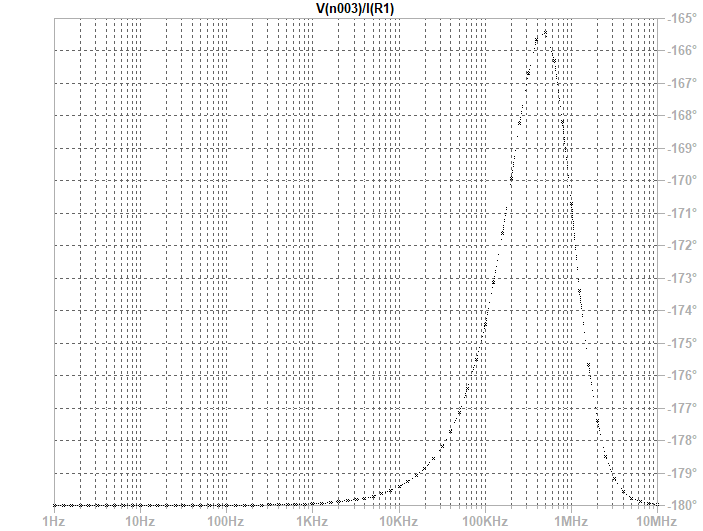
\includegraphics[scale=0.4]{Resources1a/zinpp2_sim}
\par\end{centering}
\caption{Calculo y simulación de la fase de la impedancia de entrada para el
caso 2}
\end{figure}

\begin{figure}[H]
\begin{centering}
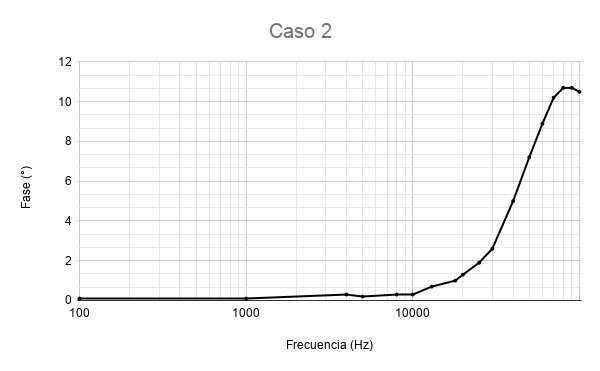
\includegraphics[scale=0.5]{Resources1a/zinpp2_med}
\par\end{centering}
\caption{Medición de la fase de la impedancia de entrada para el caso 2}

\end{figure}

\begin{figure}[H]
\begin{centering}
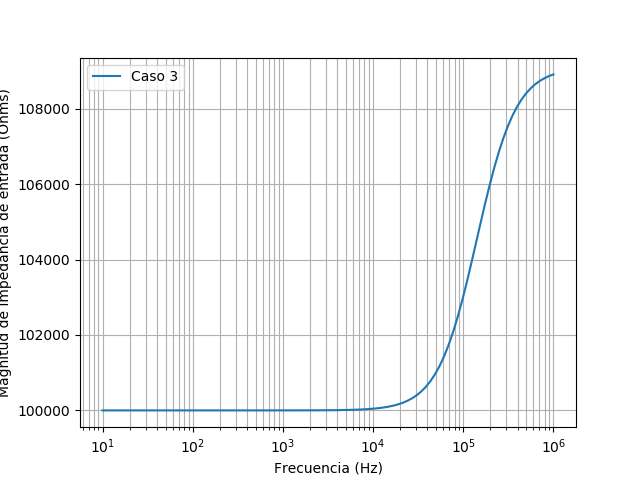
\includegraphics[scale=0.5]{Resources1a/zinpm3}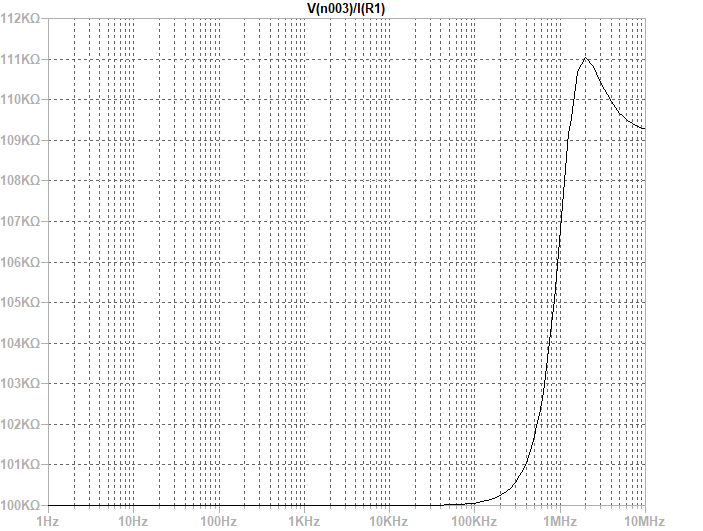
\includegraphics[scale=0.4]{Resources1a/zinpm3_sim}
\par\end{centering}
\caption{Calculo y simulación del modulo de la impedancia de entrada para el
caso 3}
\end{figure}

\begin{figure}[H]
\begin{centering}
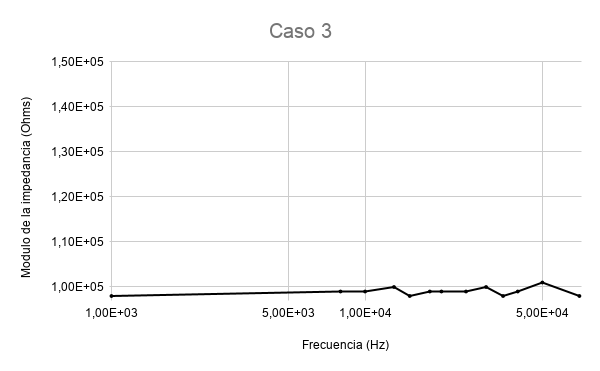
\includegraphics[scale=0.5]{Resources1a/zinpm3_med}
\par\end{centering}
\caption{Medición del modulo de la impedancia de entrada para el caso 3}

\end{figure}

\begin{figure}[H]
\begin{centering}
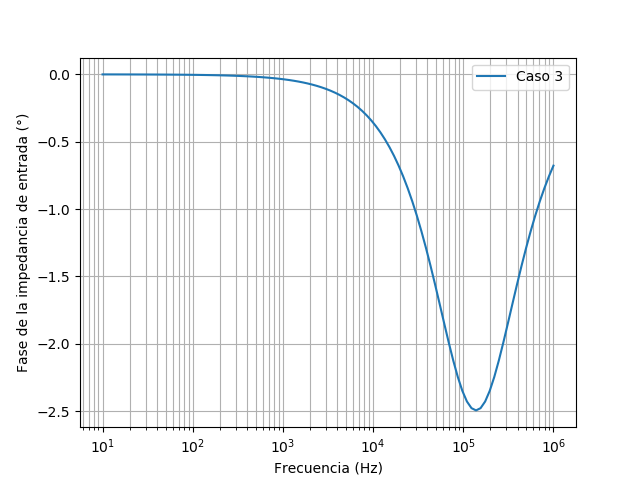
\includegraphics[scale=0.5]{Resources1a/zinpp3}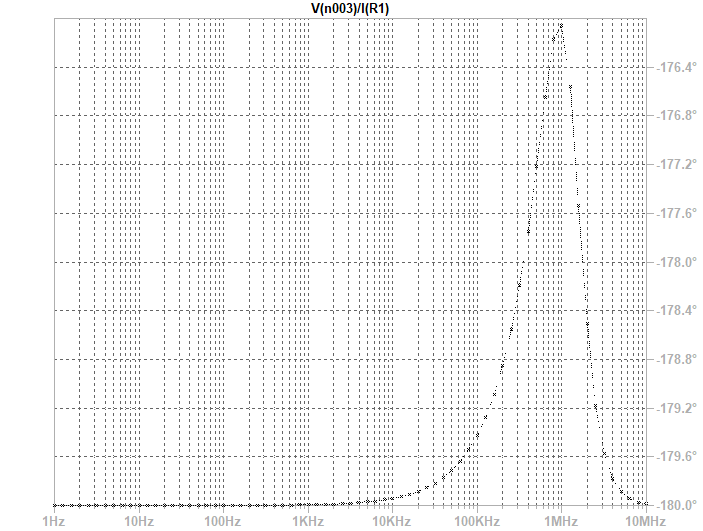
\includegraphics[scale=0.4]{Resources1a/zinpp3_sim}
\par\end{centering}
\caption{Calculo y simulación de la fase de la impedancia de entrada para el
caso 3}
\end{figure}

\begin{figure}[H]
\begin{centering}
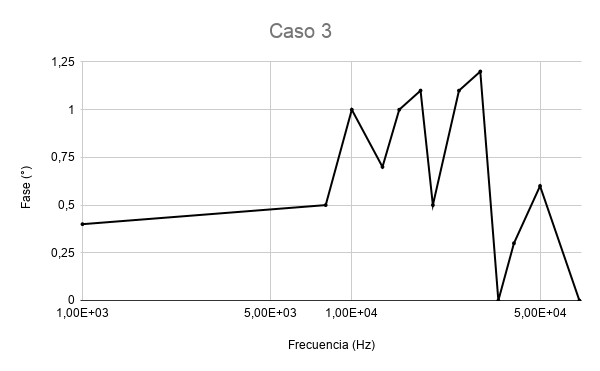
\includegraphics[scale=0.5]{Resources1a/zinpp3_med}
\par\end{centering}
\caption{Medición de la fase de la impedancia de entrada para el caso 3}

\end{figure}

Como se puede observar, en los casos 1 y 2, el modelo teórico calculado
y las simulaciones se condicen acordemente con lo medido. Las diferencias
en los valores se deben a la incertidumbre que genera el analizador
de impedancias junto con los valores que se usaron para las resistencias
del circuito (los valores nominales mas cercanos), y las toleraqncias
de dichas resistencias. No obstante, en el caso 3 se puede ver que
las diferencias entre lo teórico y lo simulado, con lo medido, son
bastante significativas, estas diferencias se deben al comportamiento
de atenuador que provee el circuito. Como a altas frecuencias las
tensiones y corrientes son altamente bajas, las mediciones tienen
un alto grado de incertidumbre debido al ruido ambiente, el cual se
hace comparable con las señales de entrada.

\subsection{Consideraciones para utilizar un modelo lineal del OpAmp}

A continuación, se decidió aclarar cuales son las consideraciones
para caracterizar a nuestro circuito de manera lineal. Para esto poseemos
varias consideraciones que son descriptas a continuación.

\subsubsection{Saturación y polo dominante}

Si tenemos en cuenta un OpAmp ideal, nuestro primer contacto con un
circuito alineal se da cuando se entra en saturación, es decir, $\left|V_{out}\right|>\left|V_{cc}\right|$.
Si consideramos una tension de entrada de la forma $V_{in}=sin(2\pi ft)$,
es decir, con amplitud \emph{1(V)} \emph{, }solo nos basta con analizar
el valor del modulo de la transferencia vista en la ecuación (\ref{eq:1_a_1}).

\[
\left|H(f)\right|\times V_{in}=\frac{R_{2}R_{3}\omega_{p}a_{0}}{\sqrt{\omega_{p}^{2}\left(-R_{1}R_{2}+R_{1}R_{3}a_{0}+R_{1}R_{3}+R_{2}R_{3}\right)^{2}+4\pi^{2}f^{2}\left(-R_{1}R_{2}+R_{1}R_{3}+R_{2}R_{3}\right)^{2}}}\times V_{in}\leq V_{cc}
\]

\[
V_{in}\leq1.3\cdot10^{-17}\sqrt{1\cdot10^{25}f^{2}+1.4\cdot10^{34}}\,\,\,Caso\,1
\]

\[
V_{in}\leq1.3\cdot10^{-16}\sqrt{2.2\cdot10^{23}f^{2}+1.4\cdot10^{34}}\,\,\,Caso\,2
\]

\[
V_{in}\leq1.3\cdot10^{-17}\sqrt{3.6\cdot10^{26}f^{2}+1.4\cdot10^{38}}\,\,\,Caso\,3
\]

Con estas ecuaciones, podemos ver, que el efecto de saturacion no
afecta en ninguno de los casos para tensiones de entrada igual a 1(V),
sin embargo, hay que tener cuidado cuando se trabaja con tensines
de entrada superiores ya que la frecuencia minima de operacion a la
cual no satura el OpAmp podria empezar a afectar nuestro circuito.

\begin{figure}[H]
\begin{centering}
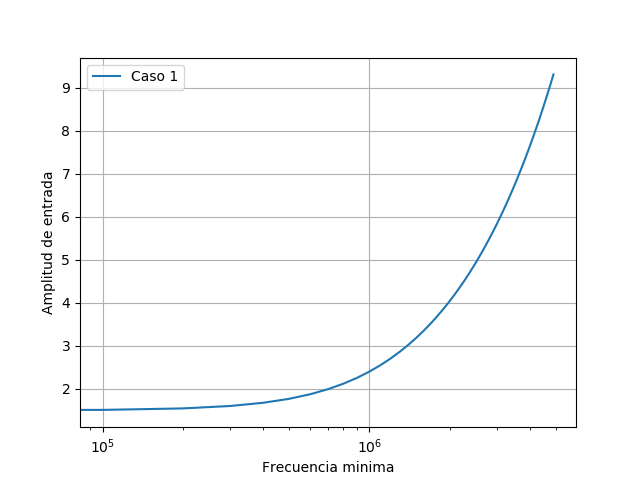
\includegraphics[scale=0.5]{Resources1a/sat1}
\par\end{centering}
\caption{Tension maxima en funcion de la frecuencia de operacion para que el
circuito no entre en saturacion caso 1}
\end{figure}

\begin{figure}[H]
\begin{centering}
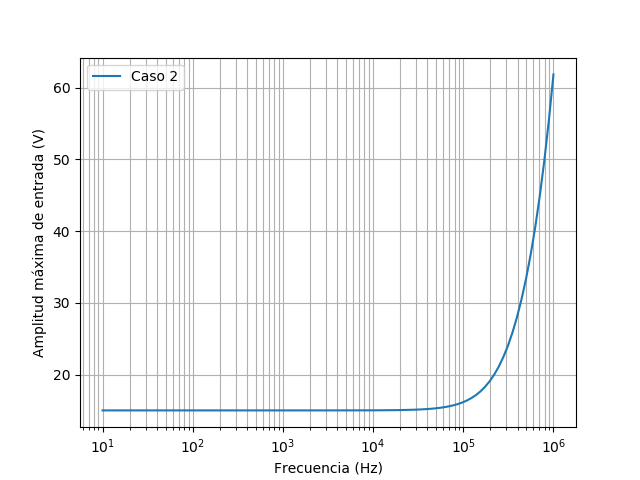
\includegraphics[scale=0.5]{Resources1a/sat2}
\par\end{centering}
\caption{Tension maxima en funcion de la frecuencia de operacion para que el
circuito no entre en saturacion caso 2}

\end{figure}

\begin{figure}[H]
\begin{centering}
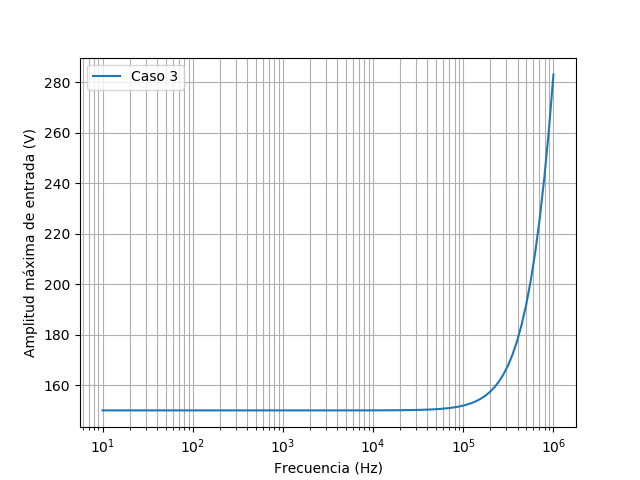
\includegraphics[scale=0.5]{Resources1a/sat3}
\par\end{centering}
\caption{Tension maxima en funcion de la frecuencia de operacion para que el
circuito no entre en saturacion caso 3}

\end{figure}

\begin{figure}[H]
\begin{centering}
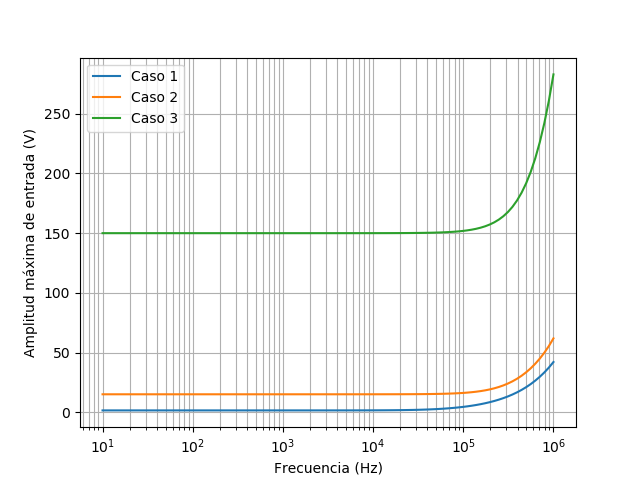
\includegraphics[scale=0.5]{Resources1a/sat123}
\par\end{centering}
\caption{Tension maxima en funcion de la frecuencia de operacion para que el
circuito no entre en saturacion}
\label{1_a_13_ggg}

\end{figure}

\begin{figure}[H]
\begin{centering}
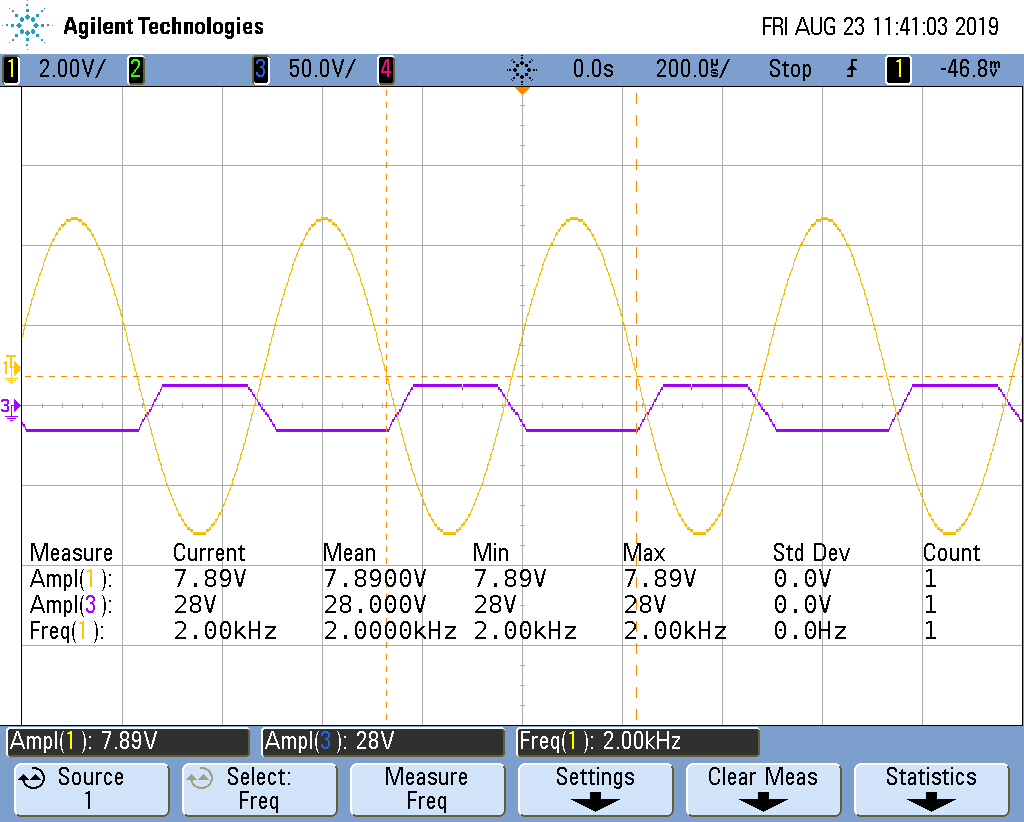
\includegraphics[scale=0.3]{Resources1a/sat1med}
\par\end{centering}
\caption{Medicion de la saturación para el caso 1 a 2(kHz)}
\label{1_a_13_asd}

\end{figure}

Como se puede ver en la figura \ref{1_a_13_asd}, el efecto de saturacion
es muy evidente ya que con una entrada de 8(Vp), si nos fijamos en
la figura \ref{1_a_21}, para 2 (kHz), la señal de entrada se encuetra
muy excedida respecto al máximo valor permitido para que no sature,
por lo tanto, la salida que se puede ver tiene 28(Vpp), que es aproximadamente
$2V_{cc}$, lo cual se condice con lo predicho. A su vez, como se
observa en la Figura \ref{1_a_13_ggg}, el efecto de saturación solo
se puede notar cuando se supera un valor de tensión practicamente
constante para cada caso en frecuencias bajas, sin embargo, en los
tres casos a frecuencias altas, la tension máxima permitida para que
empieze a haber saturación tiende a infinito, esto se da por el efecto
pasabajos del circuito, como fue explicado anteriormente.

\subsubsection{Slew Rate}

Otro problema con el cual nos topamos a la hora te poner limites a
nuestro circuito será el Slew Rate (SR), que indica el valor máximo
que puede tener $\frac{\partial V_{out}}{\partial t}$. Esto significa
que a una entrada \emph{x(t) }sinusoidal de la forma $x(t)=V_{p}sin(2\pi ft)$
le corresponde una salida $v_{out}(t)=\left|H(f)\right|V_{p}sin(2\pi ft+\phi(\omega))$
siendo $H(f)=\left|H(h)\right|e^{i\phi(\omega)}$. Por lo tanto, derivando
la salida nos queda la ecuación (\ref{eq:1_a_3}).

\begin{equation}
\frac{\partial v_{out}}{\partial t}=\left|H(f)\right|V_{p}2\pi f\,cos\left(2\pi ft+\phi(\omega)\right)\label{eq:1_a_3}
\end{equation}

A su vez, sabemos que, $cos(\alpha)\leq1$, por lo tanto;

\[
\frac{\partial v_{out}}{\partial t}\leq\left|H(f)\right|V_{p}2\pi f\leq SR
\]

\begin{equation}
f\leq\frac{SR}{\left|H(f)\right|2\pi V_{p}}\label{eq:1_a_4}
\end{equation}

\[
V_{in}\leq\frac{6.37\times10^{-4}SR\,\sqrt{62.5\times10^{3}\omega_{p}^{2}\left(R_{1}R_{2}+R_{1}R_{3}a_{0}+R_{1}R_{3}+R_{2}R_{3}\right)^{2}+2.5\times10^{6}f^{2}\left(R_{1}R_{2}+R_{1}R_{3}+R_{2}R_{3}\right)^{2}}}{R_{2}R_{3}\omega_{p}a_{0}f}
\]

Como se puede ver en la Figura \ref{1_a_13}, el valor de $SR=\frac{2.65225\,(V)}{4.75\,(\mu s)}=0.55836\left(\frac{V}{\mu s}\right)$,
por lo tanto nos queda que para cada caso se deben cumplir las siguientes
ecuaciones. Estas ecuaciones se pueden ver en la figuras \ref{1_a_4},
\ref{1_a_15} y \ref{1_a_16}.

\[
V_{in}\leq\frac{7.5\cdot10^{-14}\sqrt{1.1\cdot10^{25}f^{2}+1.4\cdot10^{34}}}{f}\,\,\,Caso\,1
\]

\[
V_{in}\leq\frac{7.5\cdot10^{-13}\sqrt{2.2\cdot10^{23}f^{2}+1.4\cdot10^{34}}}{f}\,\,\,Caso\,2
\]

\[
V_{in}\leq\frac{7.5\cdot10^{-14}\sqrt{3.6\cdot10^{26}f^{2}+1.4\cdot10^{38}}}{f}\,\,\,Caso\,3
\]

\begin{figure}[H]
\begin{centering}
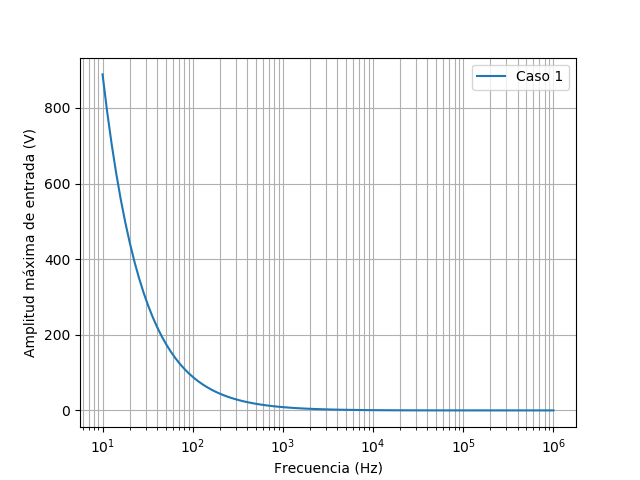
\includegraphics[scale=0.5]{Resources1a/SlewRate1}
\par\end{centering}
\caption{Calculo de tension pico maxima en funcion de la frecuencia para que
no haya slew rate Caso 1}
\label{1_a_4}

\end{figure}

\begin{figure}[H]
\begin{centering}
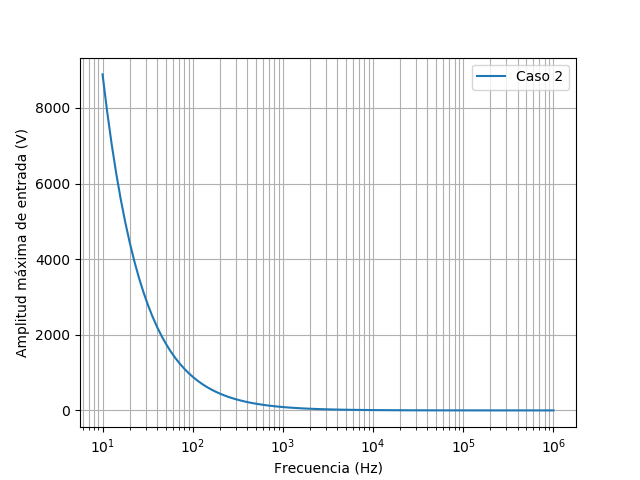
\includegraphics[scale=0.5]{Resources1a/SlewRate2}
\par\end{centering}
\caption{Calculo de tension pico maxima en funcion de la frecuencia para que
no haya slew rate Caso 2}
\label{1_a_15}

\end{figure}

\begin{figure}[H]
\begin{centering}
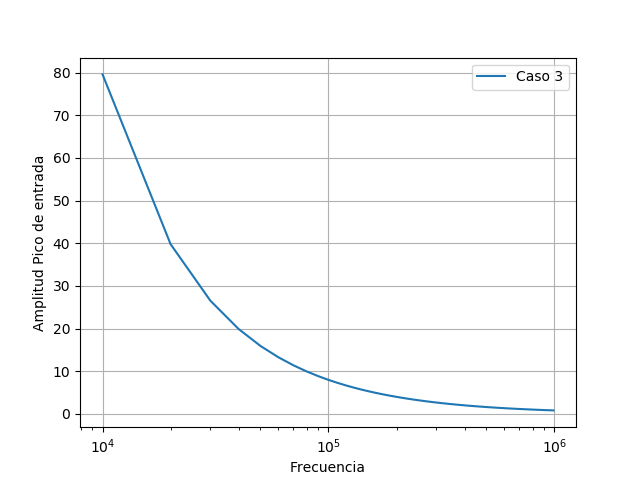
\includegraphics[scale=0.5]{Resources1a/SlewRate3}
\par\end{centering}
\caption{Calculo de tension pico maxima en funcion de la frecuencia para que
no haya slew rate Caso 3}
\label{1_a_16}

\end{figure}

\begin{figure}[H]
\begin{centering}
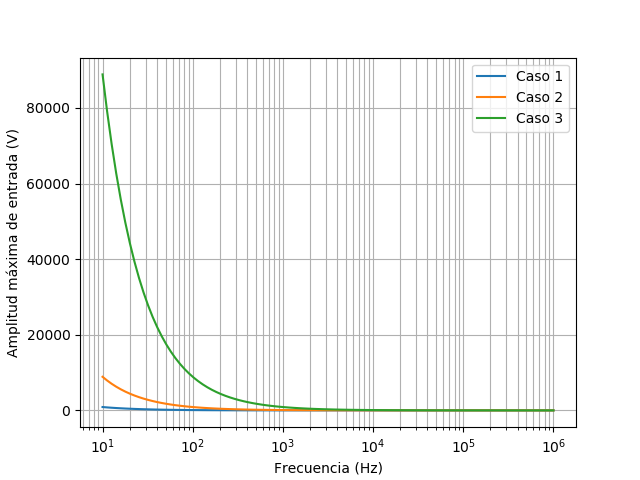
\includegraphics[scale=0.5]{Resources1a/SlewRate123}
\par\end{centering}
\caption{Calculo de tension maxima en funcion de la frecuencia para que no
haya slew rate}
\label{1_a_18}

\end{figure}

\begin{figure}[H]
\begin{centering}
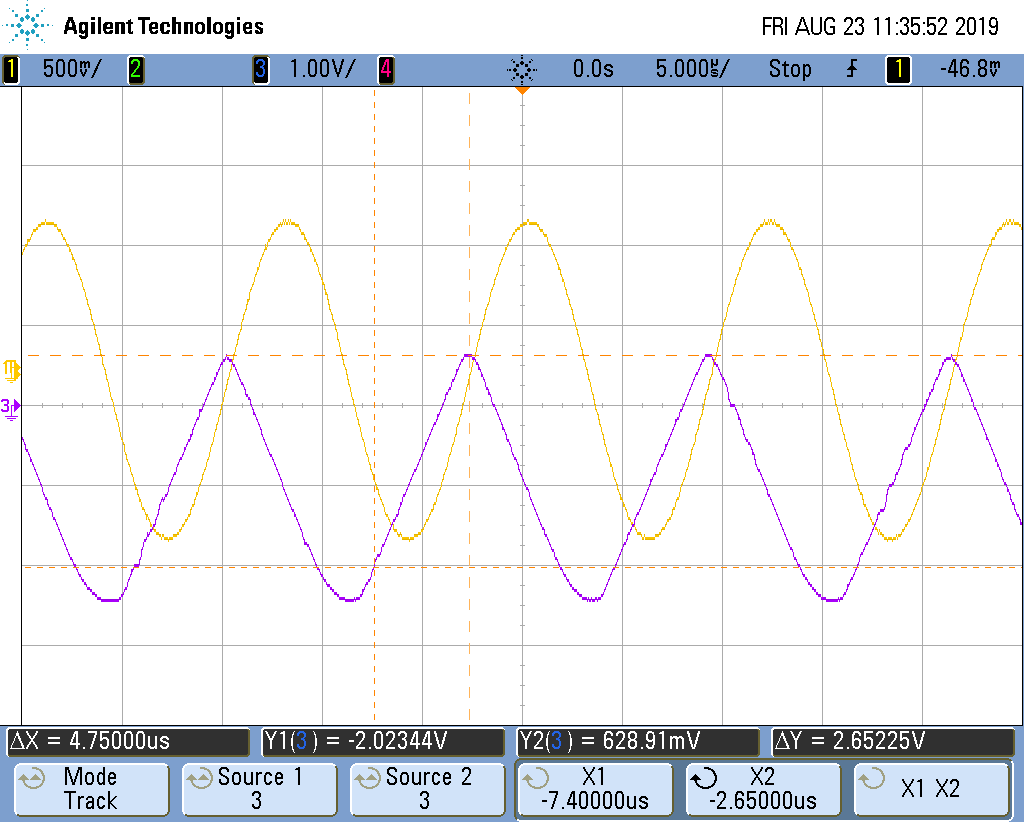
\includegraphics[scale=0.3]{Resources1a/slewRatemed}
\par\end{centering}
\caption{Medicion de la pendiente del Slew Rate}
\label{1_a_13}

\end{figure}

Como se puede observar en la Figura \ref{1_a_18}, los efectos del
\emph{slew Rate }comienzan a hacerse muy significativos a altas frecuencías,
lo cual se condice con lo explicado en la teoría. Sin embargo, los
valores picos a la entrada del circuito para frecuencias bajas, si
bien son finitos, son extremadamente grandes comparado con los valores
máximos para la saturación, por lo tanto, se deberá tener en cuenta
ambos efectos a la hora de aplicar una tension de entrada, para que
no se encuentre ninguna alinialidad en el circuito. 

\subsubsection{Crossover distortion}

La crossover distortion o distorsión de cruce por cero, es una distorsion
que se da en Amplificadores Operacionales que tienen a la salida una
etapa ``Push-Pull'', una de estas etapas se muestra en la Figura
\ref{1_a_6}. Esta alinialidad se produce por las corrientes de BIAS
de los transistores BJT en esta etapa, que generan una caida de tension
de 0.7(V), por lo tanto, la salida del circuito sera 0(V), siempre
que $\left|v_{in}\right|\leq0.7(V)$, por lo tanto, la salida del
amplificador a una estrada senoidal sera la mostrada en la Figura
\ref{1_a_7}. Como el amplificador LM324 posee una etapa push-pull,
es necesario solucionar este problema, para esto, la primera solucion
fue crear un offset a la entrada de amplitud $V_{offset}\approx V_{p}+0.7(V)$,
siendo $V_{p}$ la amplitud de la tension de entrada. De esta manera,
nos aseguramos que el minimo valor de la senoidal de entrada se encuentra
por arriba de los 0.7(V) y por lo tanto, uno de los transistores de
la etapa ``push-pull'' se mantendra siempre en modo activo, por
lo cual, no abra una zona alineal en la transferencia.

\begin{figure}[H]
\begin{centering}
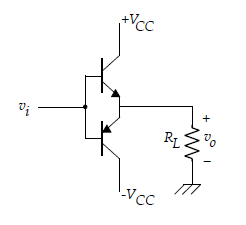
\includegraphics[scale=0.5]{Resources1a/push-pull}
\par\end{centering}
\caption{Etapa Push-Pull con transistores PNP y NPN}
\label{1_a_6}
\end{figure}

\begin{figure}[H]
\begin{centering}
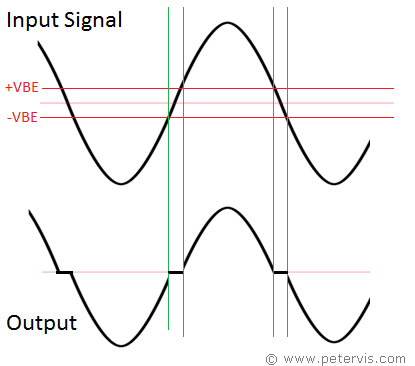
\includegraphics[scale=0.5]{Resources1a/crossover}
\par\end{centering}
\caption{Crossover Distortion}
\emph{\label{1_a_7}}
\end{figure}

\begin{figure}[H]
\begin{centering}
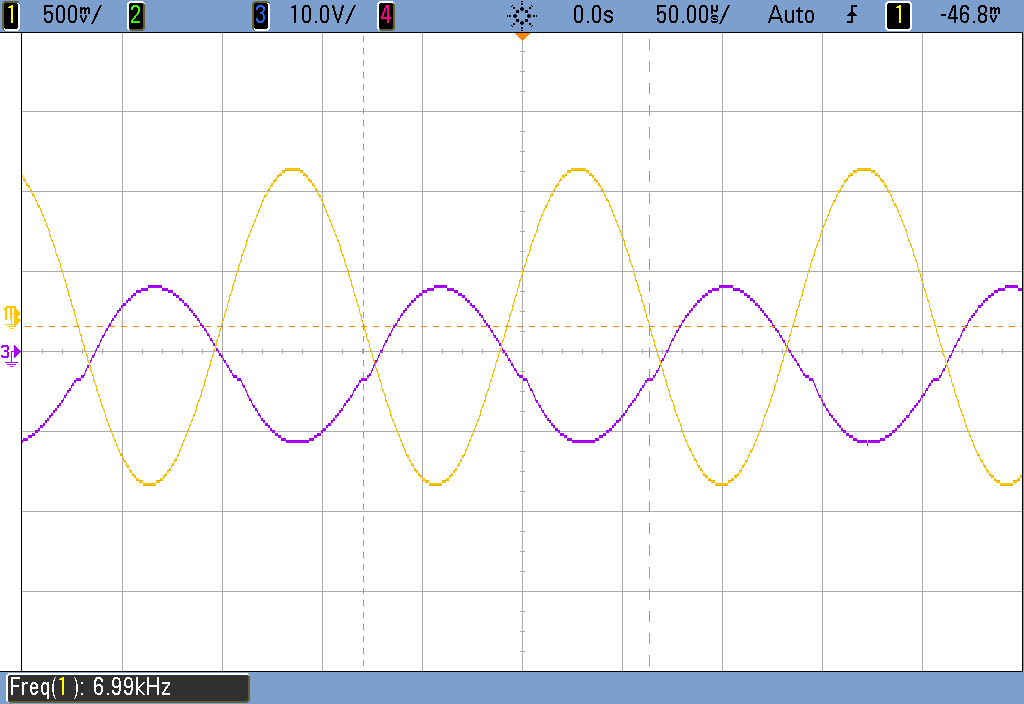
\includegraphics[scale=0.3]{Resources1a/CrossDistmed}
\par\end{centering}
\caption{Medición de la distorsión de cruce por cero}

\end{figure}

Para solucionar este problema, se decidió ingresar al circuito con
una tensión de la forma $V_{in}=A\,sin(2\pi ft)+V_{offset}$, siendo,
$V_{offstet}$ una tensión lo suficientemente grande para que alguno
de los transistores BJT de la etapa push-pull se encuentre siempre
polarizado. Sin embargo, esta solución nos afectó posteriormente a
las mediciones de la transferencia, ya que como se va a explicar en
la siguiente subseccion, la amplitud máxima de entrada al circuito
esta limitada por ciertas curvas, por lo tanto, al agregarle un offset,
estamos limitando todavía mas nuestro circuito.

\subsubsection{Conclusión}

En conclusion, teniendo en cuenta los efectos del Slew Rate y de la
saturacion para diferenctes frecuencias del espectro, los resultados
para poder medir la transferencia del circuito sin tener efectos alineales
determinan, que para cierta frecuencia elegida para medir, la amplitud
maxima de la tensíon de entrada al circuito deberá estar por debajo
de las curvas mostradas en las Figuras \ref{1_a_21}, \ref{1_a_24}
y \ref{1_a_25}.

\begin{figure}[H]
\begin{centering}
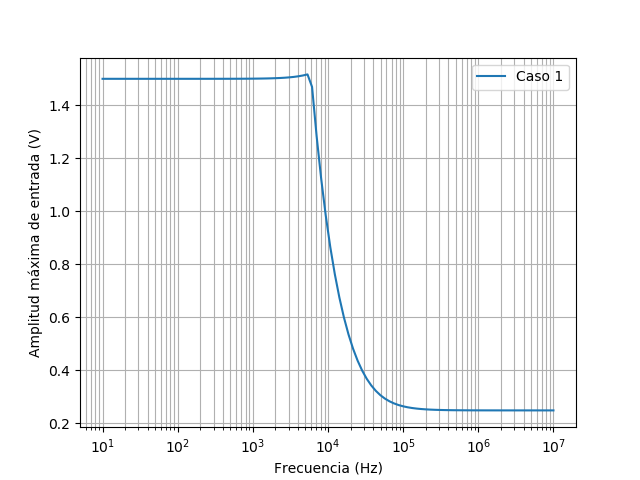
\includegraphics[scale=0.5]{Resources1a/AmplMaxVsFreq1}
\par\end{centering}
\caption{Amplitud máxima de entrada en funcion de la frecuencia para el caso
1}
\label{1_a_21}

\end{figure}

\begin{figure}[H]
\begin{centering}
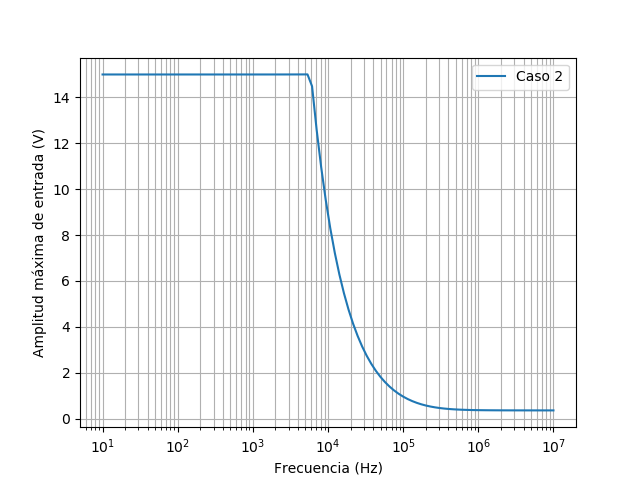
\includegraphics[scale=0.5]{Resources1a/AmplMaxVsFreq2}
\par\end{centering}
\caption{Amplitud máxima de entrada en funcion de la frecuencia para el caso
2}
\label{1_a_24}

\end{figure}

\begin{figure}[H]
\begin{centering}
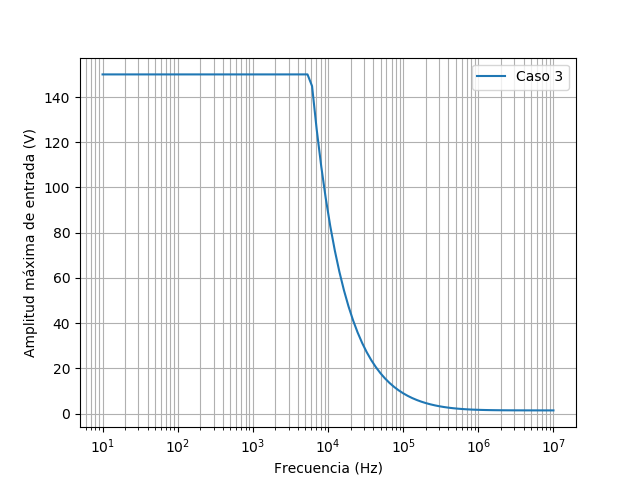
\includegraphics[scale=0.5]{Resources1a/AmplMaxVsFreq3}
\par\end{centering}
\caption{Amplitud máxima de entrada en funcion de la frecuencia para el caso
2}
\label{1_a_25}

\end{figure}

\begin{figure}[H]
\begin{centering}
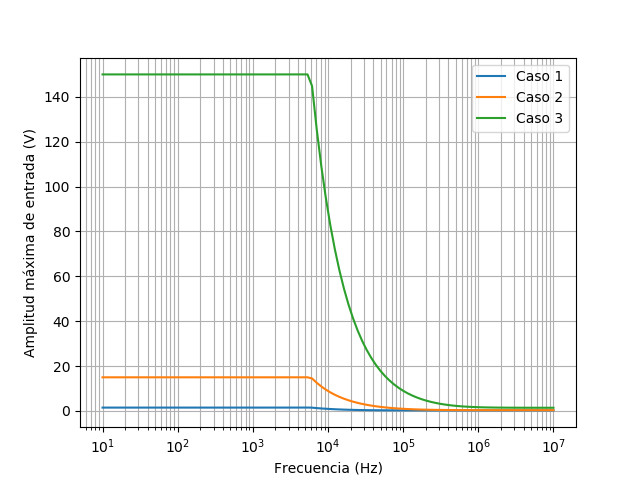
\includegraphics[scale=0.5]{Resources1a/AmplMaxVsFreq123}
\par\end{centering}
\caption{Amplitud máxima de entrada en funcion de la frecuencia}

\end{figure}

Como se puede observar, cuando la frecuencia se hace lo suficientemente
grande, la aplitud de entrada se aproxima a cero, por lo tanto, en
cada caso, se encontrará una cierta frecuencia máxima para la cual
no se podrá medir la transferencia del circuito ya que la tensión
de entrada al mismo será del orden del ruido electromagnetico ambiente
del laboratorio.

\subsection{Otros fenomenos que afectan el comportamiento del OpAmp}

\subsubsection{Corriente de BIAS y Offset de entrada}

El siguiente inconveniente se da debido a que el amplificado operacional
esta compuesto por transistores BJT internamente, por ende, cada terminal
$v^{+}$ y $v^{-}$ tiene una corriente necesaria para polarizar a
los transistores internamente que debe ser tenida en cuenta. A su
vez, debe ser tenido en cuenta el offset de entrada, que generara
una salida del tipo $V_{out}=A(\omega)\left(v^{+}-v^{-}+v_{io}\right)$
siendo $v_{io}$ la tensión de offset de entrada. En el caso del Amplificador
Operacional LM324, las caracteristicas dadas por el fabricante son
las siguientes:

\[
I_{bias}\approx45(nA)
\]
 
\[
v_{io}\approx2(mV)
\]

Sin embargo, hay que tener en cuenta que en la hoja de datos se aclara
que la corriente de Bias puede llegar a valer hasta 100 (nA) y que
la tension de offset de entrada puede llegar a valer 3 (mV), los valores
dichos previamente son valores tipicos, y estos son valores máximos.
A su vez, la corriente de offset de entrada sera:

\[
I_{io}\approx5(nA)
\]

\subsection{Aplicaciones y caracerísticas}

Como pudimos observar anteriormente, nuestro circuito es un pasabajos
inversor con un rango de frecuencias determinadas para cada caso,
durante esta sección nos centraremos en explicar algunas características
de nuestro circuito.

\subsubsection{Efecto de la resistencia R4 en el circuito inversor}

Como pudimos ver en las las subsecciones \ref{subsec:1_a_1} y \ref{subsec:1_a_2},
la transferencia y la impedancia de entrada no dependen del valor
de $R_{4}$, lo cual nos hace pregutarnos cual es el propósito de
esta resistencia. En principio, la resistencia tiene el objetivo de
cargar nuestro circuito para que funcione adecuadamente, esto querría
decir que la resistencia $R_{4}$ podría tomar cualquier valor entre
$0\,e\,\infty$, sin embargo, nuestro circuito presenta una corriente
de salida máxima y si hacemos tender $R_{4}\longrightarrow0$, la
corriente necesaria tendería a infinito, lo cual no es posible. El
otro caso posible es que $R_{4}\longrightarrow\infty$, esto significaria
que la corriente de salida del OpAmp sea la mínima, y es necesario
verificar que esa corriente no sea menor a la corriente minima de
salida del OpAmp. Sin embargo, como el segundo caso no suele traer
problemas, nos enfocaremos en procurar que la corriente de salida
no supere la corriente máxima nominal del amplificador operacional.
Para esto, y aproximando $i_{2}\approx0$, podemos decir que $R_{4}>\frac{V_{out}}{i_{max}}$.

\subsubsection{Efecto de la resistencia R3}

Por otro lado, podemos ver como, en la figura \ref{1_a_1}, la resistencia
$R_{3}$nos determina la tensión $v^{-}$. Sabiendo que $v^{+}=0(V)$,
significa que en cierta medida, la ganancia de nuestro circuito va
a estar dada por el valor de $R_{3}$ y en particular , si $R_{3}\longrightarrow0$,
entonces $v^{-}=0(v)$, por lo tanto $V_{out}=A(\omega)\,\left(v^{+}-v^{-}\right)=0(v)$,
con lo cual nuestra ganancia sería nula. De la misma manera, podemos
ver que si $R_{3}\longrightarrow\infty$, entonces la ganancia es
máxima.

\begin{figure}[H]
\begin{centering}
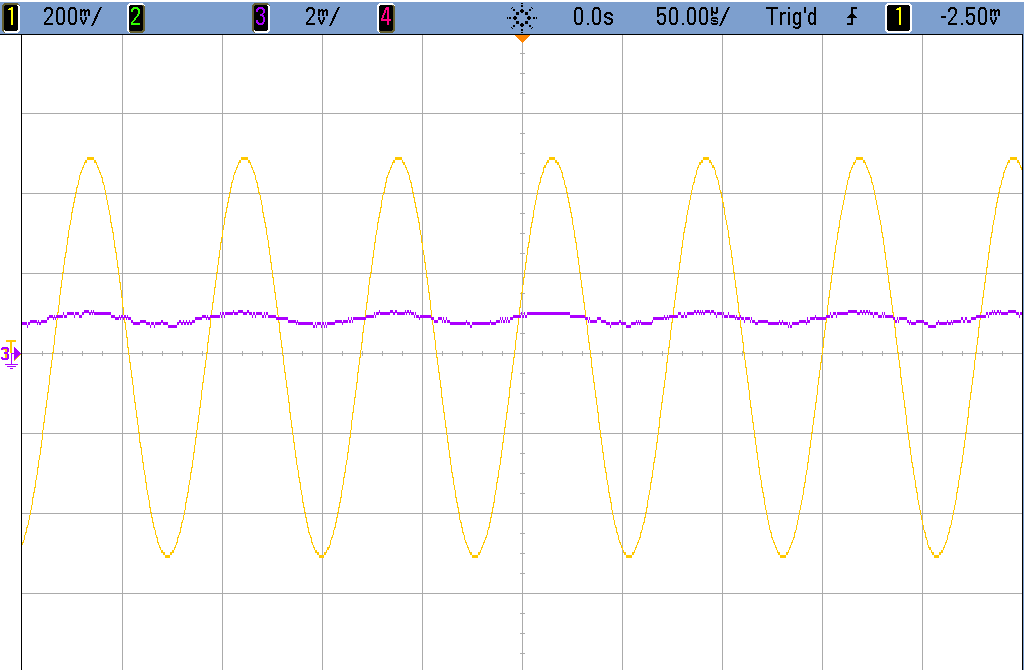
\includegraphics[scale=0.3]{Resources1a/r3=0}
\par\end{centering}
\caption{Mediciones del efecto de la resistencia R3}
\label{1_a_23}
\end{figure}

Como podemos ver en la Figura \ref{1_a_23}, la tension de salida
no es exactamente 0(V), esto se debe a la tension de offset de entrada
de la ecuación $V_{out}=A(\omega)\,\left(v^{+}-v^{-}+v_{offset}\right)=0(v)$,
esta tensión de offset de entrada se debe a las diferencias entre
los transistores de entrada, que, mediante la amplificación del amplificador
operacional, se pone en evidencia a la salida del circuito.

\subsection{DC Sweep a la entrada}

Para probar el efecto de la saturacion, se aplico un DC Sweep a la
entrada para observar la salida, lo que se observo se muestra en las
Figuras \ref{1_a_39},\ref{1_a_40} y \ref{1_a_41}.

\begin{figure}[H]
\begin{centering}
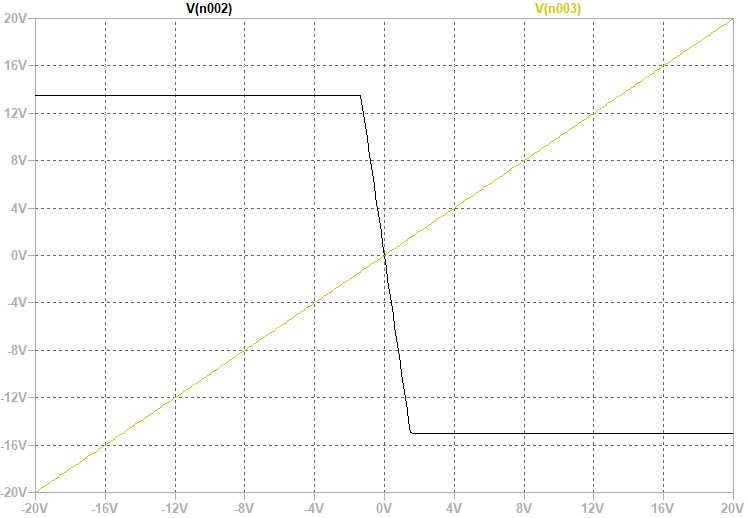
\includegraphics[scale=0.4]{Resources1a/dcswp1sim}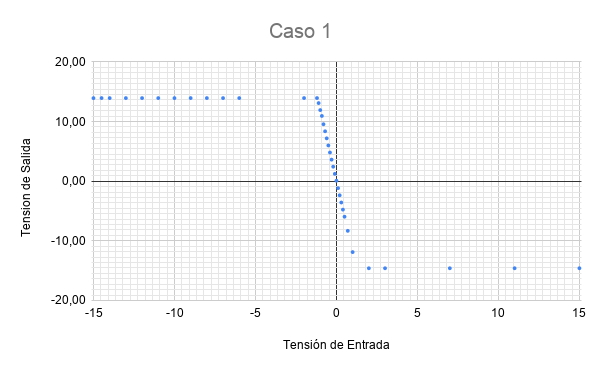
\includegraphics[scale=0.4]{Resources1a/DCSWEEP1MED}
\par\end{centering}
\caption{Simulación y mediciones del DC Sweep para el caso 1}
\label{1_a_39}

\end{figure}

\begin{figure}[H]
\begin{centering}
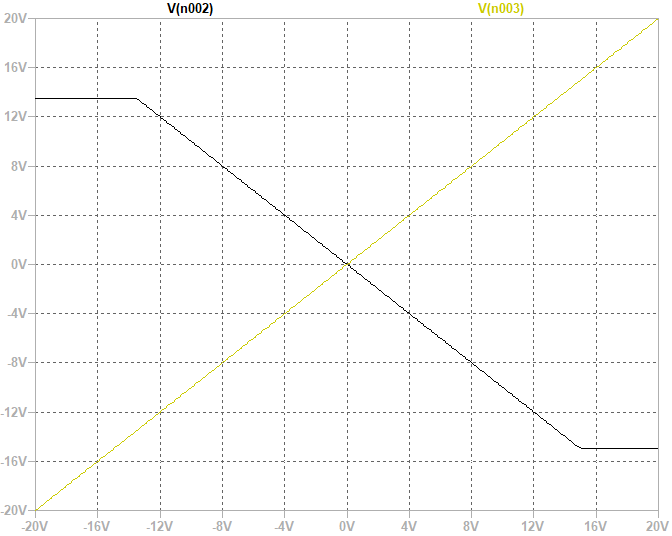
\includegraphics[scale=0.4]{Resources1a/dcswp2sim}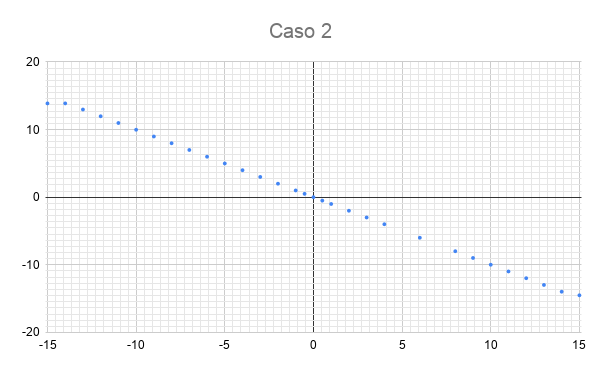
\includegraphics[scale=0.4]{Resources1a/DCSWEEP2MED}
\par\end{centering}
\caption{Simulación y mediciones del DC Sweep para el caso 2}
\label{1_a_40}

\end{figure}

\begin{figure}[H]
\begin{centering}
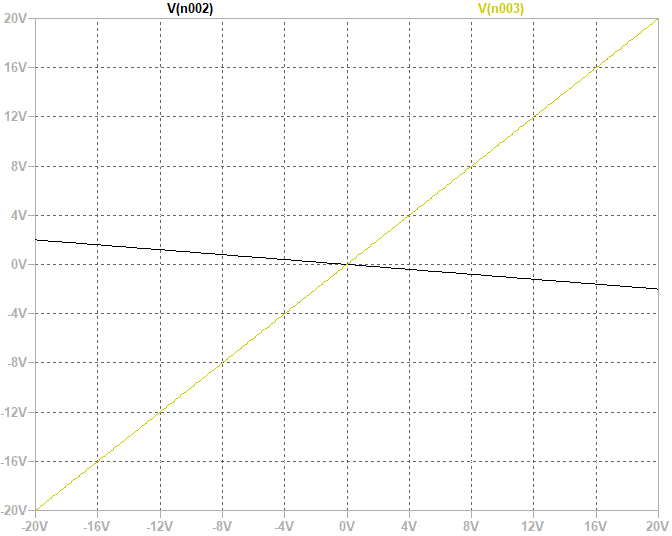
\includegraphics[scale=0.4]{Resources1a/dcswp3sim}\includegraphics[scale=0.4]{Resources1a/DCSWEEP3MED}
\par\end{centering}
\caption{Simulación y mediciones del DC Sweep para el caso 3}
\label{1_a_41}

\end{figure}

Como se puede observar, practicamente no hay diferencias entre lo
calculado y lo medido, las pequeñas diferencias en la $V_{sat}$,
se deben a que la fuente que se uso para generar una tension de $V_{cc}\,y\,-V_{cc}$,
tenia cierta impresicion. A su vez se suma la tension $V_{pol}$ de
polarizacion de los transistores de la etapa push-pull, lo que genera
que $V_{sat}\approx V_{cc}-V_{pol}$.
\end{document}
